\chapter{A prelude into topology}
\label{cha:appendix_topology}

% opening paragraph
The electronic states introduced in appendix~\ref{cha:appendix_quantum} carry both amplitudes and phases.
When we compare states at different parameter values, we must account for their relative phases.
In this appendix, we develop this connection through the Berry phase, the Berry connection, and the Berry curvature.
We then return to a group of electronic bands and establish the time-reversal properties of spinor states.
We apply these results to the band-subspace and parity analysis in chapter~\ref{cha:fundamentals_c}.

The discussion of the Berry phase, connection, and curvature partly draws on the educational video by Tony Low at the University of Minnesota Twin Cities~\cite{low2025berry}.

\newpage
\section{From phase freedom to the Berry phase}
\label{sec:berry_phase_topology}

% opening paragraph
The time-dependent Schrödinger equation describes how a quantum state evolves under a given hamiltonian.
When the hamiltonian changes slowly and returns to its initial form, the state can acquire a phase that depends on the path through parameter space.
We first derive this geometric contribution, and use it to compare electronic states at neighbouring wave vectors later.
For the application to electronic bands, we use the cell-periodic states introduced in equation~\eqref{bloch_hamiltonian_topology},
with inner products normalized over one unit cell.

\subsection{The phase of a quantum state}

We first examine the freedom to choose the phase of an individual normalized state.
For any real phase $\varphi_n(\vec{k}\,)$, we can transform the state as:

\begin{equation}
    \ket{u'_{n\vec{k}}}
    =\mathrm{e}^{\mathrm{i}\varphi_n(\vec{k}\,)}\ket{u_{n\vec{k}}}
\label{bloch_phase_freedom_topology}
\end{equation}

This replacement changes neither the band energy nor the projector
$\ket{u_{n\vec{k}}}\bra{u_{n\vec{k}}}$.
The transformed ket therefore represents the same physical state.
However, a derivative with respect to $\vec{k}$ also differentiates the chosen phase.
Consequently, we must account for this freedom when connecting states at different wave vectors.
We now examine how this freedom enters the evolution of a state and the comparison of neighbouring states.

\subsection{From adiabatic evolution to the geometric phase}
\label{subsec:adiabatic_geometric_phase_appendix}

We return to the time-dependent Schrödinger equation~\eqref{time-dependent_Schrodinger_equation}.
Let the hamiltonian depend smoothly on a set of real parameters $\vec{\lambda}(t)$.
At each instant, its normalized eigenstate satisfies:

\begin{equation}
    \hat{h}(\vec{\lambda}(t))\ket{n(t)}=E_n(t)\ket{n(t)},
    \qquad \braket{n(t)|n(t)}=1
\label{instantaneous_eigenstate_berry_appendix}
\end{equation}

here, $\ket{n(t)}$ abbreviates $\ket{n(\vec{\lambda}(t))}$.
We assume that this level remains non-degenerate and that a finite energy gap separates it from the other levels throughout the path.
Starting in $\ket{n(0)}$, we traverse a fixed smooth parameter path slowly enough to suppress transitions to other levels.
This is the adiabatic limit~\cite{berry1984quantal,xiao2010berry}.
To leading adiabatic order, we therefore write the evolving state as:

\begin{equation}
\left\{\begin{aligned}
    \ket{\Psi(t)}
    &\simeq\mathrm{e}^{\mathrm{i}\delta_n(t)}
    \mathrm{e}^{\mathrm{i}\gamma_n(t)}\ket{n(t)} \\
    \delta_n(t)&=-\frac{1}{\hbar}\int_0^t E_n(t')\,\dif t'
\end{aligned}\right.
\label{adiabatic_phase_separation_appendix}
\end{equation}

The energy and the elapsed evolution time determine the dynamical phase $\delta_n(t)$.
For a fixed hamiltonian, it gives the familiar factor $\mathrm{e}^{-\mathrm{i}E_nt/\hbar}$.
However, retaining this phase alone for a changing eigenstate gives
$\ket{\Psi_0(t)}=\mathrm{e}^{\mathrm{i}\delta_n(t)}\ket{n(t)}$ and:

\begin{equation}
    \left[\mathrm{i}\hbar\frac{\dif}{\dif t}-\hat{h}(t)\right]\ket{\Psi_0(t)}
    =\mathrm{i}\hbar\mathrm{e}^{\mathrm{i}\delta_n(t)}\frac{\dif}{\dif t}\ket{n(t)}
\label{dynamical_phase_residual_appendix}
\end{equation}

The right-hand side need not vanish.
The additional phase $\gamma_n(t)$ accounts for the change of the instantaneous eigenstate itself.
We now substitute the state with both phases into the Schrödinger equation and project onto $\bra{n(t)}$.
At the same adiabatic order, we obtain:

\begin{equation}
\begin{aligned}
    -\hbar\bigl(\dot{\delta}_n+\dot{\gamma}_n\bigr)
    +\mathrm{i}\hbar\bra{n(t)}\frac{\dif}{\dif t}\ket{n(t)}
    &=E_n(t) \\
    \dot{\gamma}_n(t)
    &=\mathrm{i}\bra{n(t)}\frac{\dif}{\dif t}\ket{n(t)}
\end{aligned}
\label{projected_adiabatic_phase_appendix}
\end{equation}

The projection determines the phase within the retained instantaneous eigenspace.
Components orthogonal to this space give the transition corrections that we neglect in the adiabatic approximation.
The single-state form in equation~\eqref{adiabatic_phase_separation_appendix} is consequently an approximate solution when the driving takes a finite time.

Using the chain rule, we now express the geometric contribution as an integral along the parameter path $C_t$:

\begin{equation}
\left\{\begin{aligned}
    \vec{\mathcal{A}}_n^{(\lambda)}(\vec{\lambda}\,)
    &\coloneqq\mathrm{i}\bra{n(\vec{\lambda}\,)}
    \nabla_{\vec{\lambda}}\ket{n(\vec{\lambda}\,)} \\
    \gamma_n(t)
    &=\mathrm{i}\int_0^t\bra{n(t')}\frac{\dif}{\dif t'}\ket{n(t')}\dif t'
    =\int_{C_t}\vec{\mathcal{A}}_n^{(\lambda)}\cdot\dif\vec{\lambda}
\end{aligned}\right.
\label{geometric_parameter_integral_appendix}
\end{equation}

here, we set $\gamma_n(0)=0$.
Traversing the same oriented path at a different rate leaves this line integral unchanged within the adiabatic description,
whereas the dynamical phase generally changes.
This explains the geometric character of $\gamma_n$.
We now take the wave vector $\vec{k}$ as the parameter and recover the same connection directly from neighbouring Bloch states.
Their comparison requires no actual time evolution of an electron.

\subsection{Connecting neighbouring states}

We first consider a single normalized band that is non-degenerate along a path.
We first identify the phase information in this single-band case, then return to a group of bands.
We choose a local gauge in which the state varies smoothly with $\vec{k}$.
For a small displacement $\dif\vec{k}$, we expand the overlap between neighbouring cell-periodic states as:

\begin{equation}
    \braket{u_{n\vec{k}}|u_{n,\vec{k}+\dif\vec{k}}}
    =1+
    \bra{u_{n\vec{k}}}\nabla_{\vec{k}}\ket{u_{n\vec{k}}}
    \cdot\dif\vec{k}
    +\mathcal{O}(|\dif\vec{k}\,|^2)
\label{neighbouring_bloch_overlap_topology}
\end{equation}

To identify this first-order change, we differentiate the normalization condition:

\begin{equation}
\begin{aligned}
    0&=\nabla_{\vec{k}}\braket{u_{n\vec{k}}|u_{n\vec{k}}} \\
    &=\bigl(\nabla_{\vec{k}}\bra{u_{n\vec{k}}}\bigr)\ket{u_{n\vec{k}}}
    +\bra{u_{n\vec{k}}}\nabla_{\vec{k}}\ket{u_{n\vec{k}}} \\
    &=2\operatorname{Re}\!\left[
    \bra{u_{n\vec{k}}}\nabla_{\vec{k}}\ket{u_{n\vec{k}}}\right]
\end{aligned}
\label{normalization_derivative_topology}
\end{equation}

The two derivative terms are complex conjugates of each other.
Their vanishing sum therefore forces the real part of
$\bra{u_{n\vec{k}}}\nabla_{\vec{k}}\ket{u_{n\vec{k}}}$ to vanish.
The first-order change of the overlap therefore carries a phase.
We describe this phase variation by introducing the Berry connection~\cite{berry1984quantal}:

\begin{equation}
    \vec{\mathcal{A}}_n(\vec{k}\,)
    \coloneqq\mathrm{i}\,
    \bra{u_{n\vec{k}}}\nabla_{\vec{k}}\ket{u_{n\vec{k}}}
\label{berry_connection_topology}
\end{equation}

here, $\nabla_{\vec{k}}$ differentiates the cell-periodic state with respect to the wave vector.
The vanishing real part of the derivative overlap makes the Berry connection real.
With $\vec{k}$ measured in inverse length, $\vec{\mathcal{A}}_n$ has the dimension of length,
and $\vec{\mathcal{A}}_n\cdot\dif\vec{k}$ is dimensionless.
Equation~\eqref{neighbouring_bloch_overlap_topology} consequently takes the form
$1-\mathrm{i}\,\vec{\mathcal{A}}_n\cdot\dif\vec{k}$ to first order.

We next substitute the phase transformation in equation~\eqref{bloch_phase_freedom_topology} into this definition.
We differentiate both the phase factor and the state, and obtain:

\begin{equation}
\begin{aligned}
    \vec{\mathcal{A}}\,'_n(\vec{k}\,)
    &=\mathrm{i}\,\mathrm{e}^{-\mathrm{i}\varphi_n(\vec{k}\,)}
    \bra{u_{n\vec{k}}}\nabla_{\vec{k}}
    \left[\mathrm{e}^{\mathrm{i}\varphi_n(\vec{k}\,)}\ket{u_{n\vec{k}}}\right] \\
    &=\vec{\mathcal{A}}_n(\vec{k}\,)-\nabla_{\vec{k}}\varphi_n(\vec{k}\,)
\end{aligned}
\label{berry_connection_gauge_transformation_topology}
\end{equation}

The Berry connection therefore depends on the phase convention, also called the gauge.
This dependence follows directly from our freedom to choose a representative for the same physical state.
For an open path from $\vec{k}_\mathrm{i}$ to $\vec{k}_\mathrm{f}$, the connection integral changes by the endpoint phases:

\begin{equation}
    \int_C\vec{\mathcal{A}}\,'_n\cdot\dif\vec{k}
    =\int_C\vec{\mathcal{A}}_n\cdot\dif\vec{k}
    -\varphi_n(\vec{k}_\mathrm{f})+\varphi_n(\vec{k}_\mathrm{i})
\label{open_path_gauge_endpoints_appendix}
\end{equation}

The integral alone is therefore gauge dependent on an open path.
We can also define an open-path geometric phase by specifying an endpoint comparison;
when the endpoint overlap is non-zero, adding its argument
$\arg\braket{u_{n\vec{k}_\mathrm{i}}|u_{n\vec{k}_\mathrm{f}}}$ cancels these endpoint changes.
For the band-topology discussion, we now consider a closed path.

\subsection{Parallel transport}

Before closing the path, we ask how to compare phases locally.
We introduce a smooth path coordinate $s$ and change the representative at each point by the accumulated connection integral:

\begin{equation}
\left\{\begin{aligned}
    \ket{\bar{u}_n(s)}
    &=\mathrm{e}^{\mathrm{i}\gamma_n(s)}\ket{u_{n\vec{k}(s)}} \\
    \gamma_n(s)&=\int_0^s\vec{\mathcal{A}}_n(\vec{k}(s'))
    \cdot\frac{\dif\vec{k}(s')}{\dif s'}\dif s' \\
    \bra{\bar{u}_n(s)}\frac{\dif}{\dif s}\ket{\bar{u}_n(s)}
    &=\mathrm{i}\frac{\dif\gamma_n}{\dif s}
    +\bra{u_{n\vec{k}(s)}}\frac{\dif}{\dif s}\ket{u_{n\vec{k}(s)}}=0
\end{aligned}\right.
\label{parallel_transport_berry_appendix}
\end{equation}

The last relation removes the local phase change between neighbouring representatives.
This relation defines parallel transport for the normalized state~\cite{xiao2010berry}.
To describe the remaining change, we abbreviate $\ket{u_n(s)}\coloneqq\ket{u_{n\vec{k}(s)}}$
and introduce the covariant derivative along the path:

\begin{equation}
\left\{\begin{aligned}
    \mathcal{A}_{n,s}&=\vec{\mathcal{A}}_n\cdot\frac{\dif\vec{k}}{\dif s},
    \qquad D_s=\frac{\dif}{\dif s}+\mathrm{i}\mathcal{A}_{n,s} \\
    D_s\ket{u_n(s)}
    &=\left[\hat{I}-\ket{u_n(s)}\bra{u_n(s)}\right]
    \frac{\dif}{\dif s}\ket{u_n(s)}
\end{aligned}\right.
\label{covariant_state_derivative_appendix}
\end{equation}

The connection subtracts the derivative component along the state itself.
Under $\ket{u'_n(s)}=\mathrm{e}^{\mathrm{i}\varphi_n(s)}\ket{u_n(s)}$,
we obtain $D'_s\ket{u'_n(s)}=\mathrm{e}^{\mathrm{i}\varphi_n(s)}D_s\ket{u_n(s)}$.
The orthogonal component can remain non-zero when the eigenspace changes.
Therefore, parallel transport fixes the local phase without requiring $D_s\ket{u_n(s)}=0$.
For a closed loop, a representative transported in this way need not return with its initial phase.

\subsection{Closing the path}

Let $C$ be an oriented closed path on which the band remains non-degenerate.
For a smooth gauge that is single-valued around this path, the Berry phase is:

\begin{equation}
    \gamma_n(C)
    =\oint_C\vec{\mathcal{A}}_n(\vec{k}\,)\cdot\dif\vec{k}
    \qquad (\mathrm{mod}\ 2\mathrm{\pi})
\label{berry_phase_closed_path_topology}
\end{equation}

Under equation~\eqref{berry_connection_gauge_transformation_topology},
the change in $\gamma_n(C)$ is the negative of the phase change accumulated around the loop.
For a single-valued gauge transformation, this change is an integer multiple of $2\mathrm{\pi}$.
This transformation therefore leaves $\mathrm{e}^{\mathrm{i}\gamma_n(C)}$ unchanged.
The local phase choices cancel, while the phase accumulated by connecting the states around the loop remains.
In particular, a smooth periodic representative obeys
$\ket{u_{n\vec{k}(s_\mathrm{f})}}=\ket{u_{n\vec{k}(0)}}$ after the endpoint identification.
Equation~\eqref{parallel_transport_berry_appendix} then gives
$\ket{\bar{u}_n(s_\mathrm{f})}=\mathrm{e}^{\mathrm{i}\gamma_n(C)}\ket{\bar{u}_n(0)}$.
This phase mismatch is the holonomy of parallel transport around the loop.
A parallel-transported representative is also periodic only when the Berry phase vanishes modulo $2\mathrm{\pi}$.

We next recover the same cancellation by discretizing the path into $M$ points.
We identify the endpoint with the starting point and write:

\begin{equation}
    \gamma_n(C)
    =-\lim_{M\rightarrow\infty}\arg
    \prod_{j=0}^{M-1}
    \braket{u_{n\vec{k}_j}|u_{n\vec{k}_{j+1}}}
    \qquad (\mathrm{mod}\ 2\mathrm{\pi})
\label{berry_phase_overlap_product_topology}
\end{equation}

here, we consistently identify the endpoint state with the initial state,
using equation~\eqref{reciprocal_lattice_identification_topology} if the loop crosses a Brillouin-zone boundary.
The mesh must be fine enough that successive overlaps are non-zero.
Every local phase then appears once in a bra and once in a ket, so it cancels from the product.
The minus sign follows from the convention in equation~\eqref{berry_connection_topology}.
At a finite mesh spacing, the overlap product generally has a magnitude smaller than unity.
Its argument gives the phase; the magnitude is not an additional phase contribution.
Equation~\eqref{neighbouring_bloch_overlap_topology} recovers the connection integral as the spacing tends to zero.

We illustrate this cancellation with four points on the same closed path in figure~\ref{fig:phase_gauge_appendix}.
For brevity, we denote the states by $\ket{u_j}\coloneqq\ket{u_{n\vec{k}_j}}$ and their overlap product by
$Z_C\coloneqq\prod_{j=0}^{3}\braket{u_j|u_{j+1}}$, with $\ket{u_4}=\ket{u_0}$ after the endpoint identification.
The green points specify the wave vectors, while the orange pointers show the extra phase factors chosen for the state representatives.
In panel (a), these factors are all unity; in panel (b), we replace each representative by $\ket{u'_j}=\mathrm{e}^{\mathrm{i}\varphi_j}\ket{u_j}$.
The pointers therefore describe phase choices, rather than spin directions or real-space vectors.
Each overlap acquires the factor $\mathrm{e}^{\mathrm{i}(\varphi_{j+1}-\varphi_j)}$.
For a consistent closed-loop choice, $\mathrm{e}^{\mathrm{i}\varphi_4}=\mathrm{e}^{\mathrm{i}\varphi_0}$, and the product of these factors is unity.
Consequently, the two choices give the same $Z_C$ and the same closed-loop phase.

\begin{figure}[htbp]
    \centering
    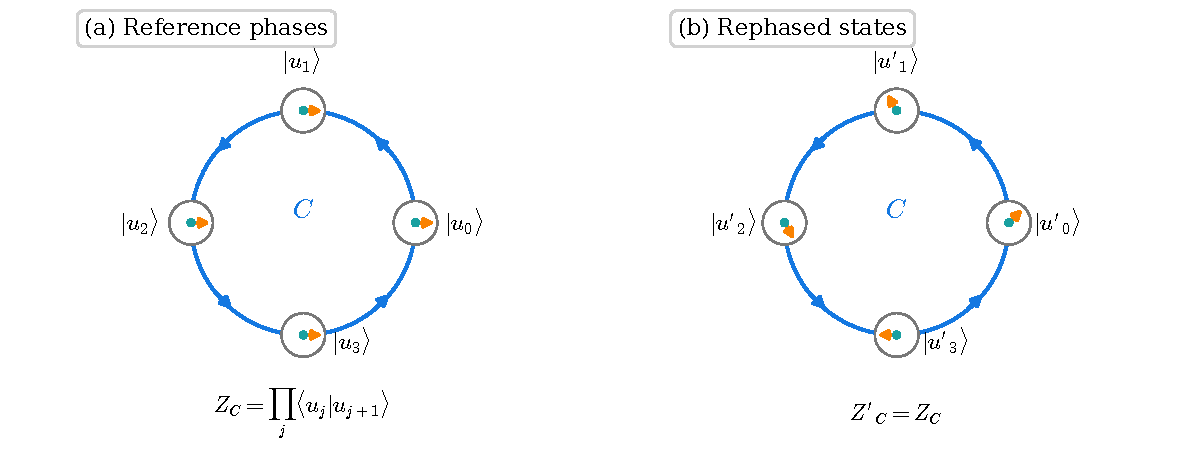
\includegraphics[width=0.8\textwidth]{figures_topo/C.1_phase_gauge.pdf}
    \caption{Two phase conventions along the same closed parameter path: (a) original representatives and (b) locally rephased representatives.}
    \label{fig:phase_gauge_appendix}
\end{figure}

The Berry phase describes the geometry of the electronic states along a chosen loop.
Here, following the loop means comparing stationary states at successive wave vectors;
we do not need to prescribe an actual time evolution of the electron.
Changing the arbitrary phase of each state leaves the closed-loop result unchanged,
whereas a smooth change of the hamiltonian or the loop can change $\mathrm{e}^{\mathrm{i}\gamma_n(C)}$ continuously,
provided the band remains non-degenerate along the loop.
The phase $\gamma_n(C)$ is not generally restricted to $0$ or $\mathrm{\pi}$,
and a Berry phase on an arbitrary loop is not by itself the two-dimensional $Z_2$ index.
The additional structure needed for that index comes from time-reversal symmetry and the full selected band subspace.

\subsection{From the Berry connection to the Berry curvature}
\label{subsec:berry_curvature_appendix}

The closed-loop phase compares states around a finite path.
We now ask how to describe this geometric information locally over a surface.
For a smooth non-degenerate band, we define the Berry curvature through the antisymmetric derivatives of the connection~\cite{xiao2010berry}:

\begin{equation}
\begin{aligned}
    \mathcal{F}_{n,ij}
    &\coloneqq\partial_{k_i}\mathcal{A}_{n,j}
    -\partial_{k_j}\mathcal{A}_{n,i} \\
    &=\mathrm{i}\left[
    \braket{\partial_{k_i}u_{n\vec{k}}|\partial_{k_j}u_{n\vec{k}}}
    -\braket{\partial_{k_j}u_{n\vec{k}}|\partial_{k_i}u_{n\vec{k}}}
    \right]
\end{aligned}
\label{abelian_berry_curvature_appendix}
\end{equation}

here, $\ket{\partial_{k_i}u_{n\vec{k}}}$ denotes $\partial_{k_i}\ket{u_{n\vec{k}}}$.
Under a smooth gauge transformation, the additional mixed derivatives of $\varphi_n$ cancel, giving $\mathcal{F}'_{n,ij}=\mathcal{F}_{n,ij}$.
Thus the single-band curvature is gauge invariant even though the connection depends on the gauge.
For an oriented surface $S$ in the $(k_x,k_y)$ plane, Stokes' theorem gives:

\begin{equation}
    \gamma_n(\partial S)
    =\oint_{\partial S}\vec{\mathcal{A}}_n\cdot\dif\vec{k}
    =\int_S\mathcal{F}_{n,xy}\dif k_x\dif k_y
    \qquad (\mathrm{mod}\ 2\mathrm{\pi})
\label{berry_curvature_stokes_appendix}
\end{equation}

This expression assumes that the band remains non-degenerate on the surface and that a smooth gauge is available over it.
The surface orientation fixes the boundary orientation.
For a sufficiently small loop, the curvature consequently gives the geometric phase per oriented area.
A loop winding around the periodically identified Brillouin zone need not bound such a surface within that zone;
equation~\eqref{berry_phase_closed_path_topology} still defines its phase, but the surface expression requires this additional check.

\subsection{The curvature in different dimensions}

In three-dimensional parameter space, we can express the same curvature as a vector:

\begin{equation}
\left\{\begin{aligned}
    \vec{\Omega}_n&=\nabla_{\vec{k}}\times\vec{\mathcal{A}}_n \\
    \Omega_{n,x}&=\mathcal{F}_{n,yz} \\
    \Omega_{n,y}&=\mathcal{F}_{n,zx}=-\mathcal{F}_{n,xz} \\
    \Omega_{n,z}&=\mathcal{F}_{n,xy}
\end{aligned}\right.
\label{berry_curvature_vector_appendix}
\end{equation}

Equivalently, $\Omega_{n,i}=\frac{1}{2}\sum_{j,l}\varepsilon_{ijl}\mathcal{F}_{n,jl}$,
where $\varepsilon_{ijl}$ is the Levi--Civita symbol in a right-handed coordinate system.
In two dimensions, $\mathcal{F}_{n,xy}$ is the perpendicular curvature component.
The relation resembles $\vec{B}=\nabla_{\vec{r}}\times\vec{A}_\mathrm{EM}$ in electrodynamics:
the connection plays the role of a vector potential, while the curvature plays the role of its field strength.
Adding a gradient changes the potential but leaves its curl unchanged.
Here, the field describes the electronic states in parameter space; the parameter space itself can be flat~\cite{xiao2010berry}.

For an arbitrary number of parameters, differential forms express the line and surface elements directly~\cite{hassani2013mathematical}.
Denoting the corresponding one-form and two-form by $\mathcal{A}_n$ and $\mathcal{F}_n$, we write:

\begin{equation}
\left\{\begin{aligned}
    \mathcal{A}_n&=\sum_i\mathcal{A}_{n,i}\dif k_i \\
    \mathcal{F}_n&=\dif\mathcal{A}_n
    =\sum_{i<j}\mathcal{F}_{n,ij}\dif k_i\wedge\dif k_j
\end{aligned}\right.
\label{berry_differential_forms_appendix}
\end{equation}

here, $\dif$ acting on a form denotes the exterior derivative.
The wedge product represents an oriented area element:
$\dif k_i\wedge\dif k_j=-\dif k_j\wedge\dif k_i$ and $\dif k_i\wedge\dif k_i=0$.
These forms collect the same components used above;
integrating the one-form along a boundary or the two-form over its surface gives equation~\eqref{berry_curvature_stokes_appendix}.

\subsection{The curvature from a projector}

The phase freedom in equation~\eqref{bloch_phase_freedom_topology} leaves the single-state projector
$\hat{\mathcal{P}}_n=\ket{u_{n\vec{k}}}\bra{u_{n\vec{k}}}$ unchanged.
This projector alone consequently cannot determine the gauge-dependent connection.
We differentiate $\hat{\mathcal{P}}_n^2=\hat{\mathcal{P}}_n$ and use its constant unit trace to obtain:

\begin{equation}
\left\{\begin{aligned}
    \operatorname{Tr}\!\left[\hat{\mathcal{P}}_n\partial_{k_i}\hat{\mathcal{P}}_n\right]
    &=\frac{1}{2}\partial_{k_i}\operatorname{Tr}\hat{\mathcal{P}}_n^2=0 \\
    \mathcal{F}_{n,ij}
    &=\mathrm{i}\operatorname{Tr}\!\left[
    \hat{\mathcal{P}}_n[\partial_{k_i}\hat{\mathcal{P}}_n,\partial_{k_j}\hat{\mathcal{P}}_n]\right]
\end{aligned}\right.
\label{projector_berry_curvature_appendix}
\end{equation}

here, the trace is over the state space.
Substituting the differentiated ket--bra product into the second line, we recover equation~\eqref{abelian_berry_curvature_appendix}.
The projector therefore determines the curvature, while a connection additionally requires a choice of phase.

\subsection{A two-component example}
\label{subsec:berry_two_component_example_appendix}

We now apply these definitions to two orthonormal basis states $\ket{\uparrow}$ and $\ket{\downarrow}$.
We keep this basis fixed throughout the calculation.
For angular parameters $\theta$ and $\varphi$, we introduce the normalized state and hamiltonian:

\begin{equation}
\left\{\begin{aligned}
    \ket{v(\theta,\varphi)}
    &=\cos\frac{\theta}{2}\ket{\uparrow}
    +\mathrm{e}^{\mathrm{i}\varphi}\sin\frac{\theta}{2}\ket{\downarrow} \\
    \hat{h}(\theta,\varphi)
    &=\frac{\Delta}{2}\left[\hat{I}-2\ket{v(\theta,\varphi)}\bra{v(\theta,\varphi)}\right],
    \qquad \Delta>0
\end{aligned}\right.
\label{two_component_berry_state_appendix}
\end{equation}

The state $\ket{v}$ has energy $-\Delta/2$, while its orthogonal partner has energy $\Delta/2$.
The level separation therefore stays finite as the parameters change.
The angles specify this illustrative hamiltonian; they are independent of the crystal wave vectors used in the thesis calculations.
We evaluate the two derivatives and obtain:

\begin{equation}
\left\{\begin{aligned}
    \bra{v}\partial_\theta\ket{v}
    &=-\frac{1}{2}\cos\frac{\theta}{2}\sin\frac{\theta}{2}
    +\frac{1}{2}\sin\frac{\theta}{2}\cos\frac{\theta}{2}=0 \\
    \bra{v}\partial_\varphi\ket{v}
    &=\mathrm{i}\sin^2\frac{\theta}{2} \\
    \mathcal{A}_\theta&=0 \\
    \mathcal{A}_\varphi&=-\sin^2\frac{\theta}{2} \\
    \mathcal{F}_{\theta\varphi}
    &=\partial_\theta\mathcal{A}_\varphi-\partial_\varphi\mathcal{A}_\theta
    =-\frac{1}{2}\sin\theta
\end{aligned}\right.
\label{two_component_berry_derivatives_appendix}
\end{equation}

here, $\mathcal{A}_\varphi$ is the coefficient of $\dif\varphi$ in the connection integral.
For a loop at fixed $\theta=\theta_0$, traversed with $\varphi$ increasing from $0$ to $2\mathrm{\pi}$, we obtain:

\begin{equation}
    \gamma(C)
    =\int_0^{2\mathrm{\pi}}\mathcal{A}_\varphi(\theta_0)\dif\varphi
    =-2\mathrm{\pi}\sin^2\frac{\theta_0}{2}
    =-\mathrm{\pi}(1-\cos\theta_0)
    \qquad (\mathrm{mod}\ 2\mathrm{\pi})
\label{two_component_berry_phase_appendix}
\end{equation}

Integrating $\mathcal{F}_{\theta\varphi}$ over the cap $0\leq\theta\leq\theta_0<\mathrm{\pi}$, we recover the same result.
The chosen state is smooth over this cap; at the south pole $\theta=\mathrm{\pi}$, we must choose a different phase convention to remove its dependence on $\varphi$.
At $\theta_0=\mathrm{\pi}/2$, the phase is $-\mathrm{\pi}$, although the state representative returns to itself after a full turn.
Its parallel-transported representative instead returns with the factor $\mathrm{e}^{-\mathrm{i}\mathrm{\pi}}=-1$.
The example therefore connects the local connection and curvature to the closed-loop phase.
It also shows why a geometric phase can vary continuously with the path while the two levels remain separated.

We now represent the same example geometrically.
For the state in equation~\eqref{two_component_berry_state_appendix}, the expectation values of the Pauli operators define a unit vector:

\begin{equation}
\left\{\begin{aligned}
    n_i&=\bra{v}\hat{\sigma}_i\ket{v},\qquad i=x,y,z \\
    \vec{n}&=(\sin\theta\cos\varphi,\sin\theta\sin\varphi,\cos\theta)
\end{aligned}\right.
\label{two_component_state_sphere_appendix}
\end{equation}

here, $\hat{\sigma}_i$ are the Pauli operators in the fixed basis $\ket{\uparrow}$ and $\ket{\downarrow}$.
The vector $\vec{n}$ specifies a point on the unit sphere, often called the Bloch sphere.
Multiplying $\ket{v}$ by an overall phase leaves all three expectation values unchanged,
so one point represents a normalized state up to this phase freedom.
This sphere describes the two-component state; its coordinates are not the crystal wave vector or the real-space position of an electron.

For a second path, we choose $\theta_0=\mathrm{\pi}/3$, as shown in figure~\ref{fig:geometric_phase_appendix}(a).
The blue arrows show the direction of increasing $\varphi$ along the boundary of the shaded northern cap.
We relate the solid angle of this cap to the geometric phase through:

\begin{equation}
    \Omega_S=2\mathrm{\pi}(1-\cos\theta_0)=\mathrm{\pi},
    \qquad \gamma(C)=-\frac{\Omega_S}{2}=-\frac{\mathrm{\pi}}{2}
    \qquad (\mathrm{mod}\ 2\mathrm{\pi})
\label{two_component_solid_angle_appendix}
\end{equation}

Since the sphere has unit radius, this solid angle is also the surface area of the shaded cap.
Along this path, the chosen representative gives $\gamma(\varphi)=-\varphi\sin^2(\theta_0/2)$.
The factor $\mathrm{e}^{\mathrm{i}\gamma(\varphi)}$ therefore moves clockwise from $1$ to $-\mathrm{i}$ in the complex plane, as shown in panel (b).
Although $\ket{v(\theta_0,2\mathrm{\pi})}=\ket{v(\theta_0,0)}$, the parallel-transported representative
$\ket{\bar{v}(\varphi)}=\mathrm{e}^{\mathrm{i}\gamma(\varphi)}\ket{v(\theta_0,\varphi)}$
returns with $\ket{\bar{v}(2\mathrm{\pi})}=-\mathrm{i}\ket{\bar{v}(0)}$.
The path thus closes on the state sphere while retaining the phase mismatch described earlier.

\begin{figure}[htbp]
    \centering
    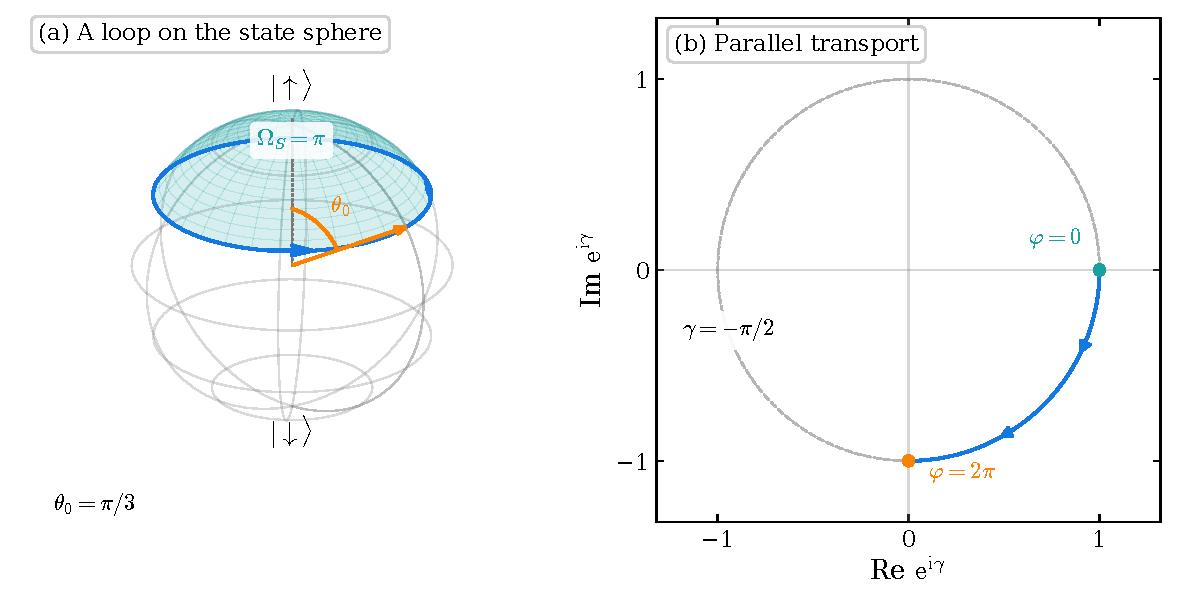
\includegraphics[width=0.8\textwidth]{figures_topo/C.2_geometric_phase.pdf}
    \caption{Geometric phase for $\theta_0=\mathrm{\pi}/3$: (a) the closed path on the state sphere and (b) the corresponding phase factor during parallel transport.}
    \label{fig:geometric_phase_appendix}
\end{figure}

\subsection{A connection to transverse transport}

The curvature also enters the motion of electrons under an external field.
We consider a wave packet in an isolated band under a weak electric field and zero magnetic field.
Its equations of motion read~\cite{sundaram1999wave,xiao2010berry}:

\begin{equation}
\left\{\begin{aligned}
    \hbar\dot{\vec{k}}&=-e\vec{E} \\
    \dot{\vec{r}}&=\frac{1}{\hbar}\nabla_{\vec{k}}E_{n\vec{k}}
    -\dot{\vec{k}}\times\vec{\Omega}_n
\end{aligned}\right.
\label{berry_anomalous_velocity_appendix}
\end{equation}

here, the electron charge is $-e$, with $e>0$.
The curvature term produces a velocity perpendicular to the electric field.
In two dimensions, we sum its charge-current contribution over occupied states and obtain:

\begin{equation}
    \sigma_{xy}^{\mathrm{int}}
    =-\frac{e^2}{\hbar}\sum_n\int_\mathrm{BZ}
    \frac{\dif^2k}{(2\mathrm{\pi})^2}\,
    f_{n\vec{k}}\Omega_{n,z}(\vec{k}\,)
\label{intrinsic_hall_curvature_appendix}
\end{equation}

here, $j_x=\sigma_{xy}^{\mathrm{int}}E_y$ fixes the sign convention,
and $f_{n\vec{k}}$ is the Fermi--Dirac occupation.
This is the intrinsic Hall contribution; the ordinary Hall effect also involves the Lorentz force from a real magnetic field.
For an isolated band, the integrated curvature defines a Chern number.
For a band insulator at zero temperature, the Hall expression then reduces to:

\begin{equation}
    C_n=\frac{1}{2\mathrm{\pi}}\int_\mathrm{BZ}\Omega_{n,z}\dif^2k\in\mathbb{Z},
    \qquad \sigma_{xy}^{\mathrm{int}}=-\frac{e^2}{h}\sum_{n\,\mathrm{filled}}C_n
\label{chern_hall_relation_appendix}
\end{equation}

The integer counts the winding of phase transformations joining local gauges over the Brillouin zone.
During a smooth deformation, this integer can change only when the band loses its isolation.
For a band insulator with broken time-reversal symmetry, this relation describes the quantized anomalous Hall response.
With a magnetic field, the corresponding analysis uses magnetic bands.
Time-reversal-related states instead cancel their contributions to the intrinsic charge Hall conductivity.
They can still contribute to a spin Hall response, whose matrix elements involve the spin-current operator;
with spin-orbit coupling, this is not generally the difference of two independent spin-channel curvatures.
These examples explain the physical role of the curvature~\cite{xiao2010berry}.
The time-reversal invariant $Z_2$ index used in this thesis requires the full band subspace, to which we now return.

\subsection{From an individual band to a band subspace}

The single-band discussion assumes that the state can be followed separately from all other states along the path.
For spinful time-reversal-symmetric systems, degeneracies are instead part of the problem.
Within a degenerate group, the hamiltonian alone does not select a unique state to follow.
Different choices can mix these states, rather than merely change their individual phases.
An individual-band Berry phase is therefore not fixed by the degenerate subspace alone.
We return to the projector in equation~\eqref{band_subspace_projector_topology}.

Within its $2N_\mathrm{p}$-dimensional subspace, we may choose a different orthonormal basis:

\begin{equation}
\left\{\begin{aligned}
    \ket{u'_{a\vec{k}}}
    &=\sum_{n=1}^{2N_\mathrm{p}}
    \ket{u_{n\vec{k}}}U_{na}(\vec{k}\,) \\
    U^\dagger(\vec{k}\,)U(\vec{k}\,)&=I \\
    \sum_{a=1}^{2N_\mathrm{p}}\ket{u'_{a\vec{k}}}\bra{u'_{a\vec{k}}}
    &=\hat{\mathcal{P}}(\vec{k}\,)
\end{aligned}\right.
\label{band_subspace_basis_transformation_topology}
\end{equation}

here, $U(\vec{k}\,)$ is a unitary matrix and $I$ is the identity matrix within the selected subspace.
The transformed basis need not diagonalize the hamiltonian when it mixes states of different energies.
Nevertheless, it describes the same projector and therefore the same band subspace.
This is the multi-state counterpart of the phase freedom introduced earlier.

We illustrate this freedom with a two-dimensional plane in a real three-dimensional inner-product space in figure~\ref{fig:subspace_basis_appendix}.
The blue vectors $\ket{1}$ and $\ket{2}$ form one orthonormal basis for the shaded plane.
Rotating both vectors through the same angle $\alpha=\mathrm{\pi}/5$ within the plane gives the orange basis $\ket{1'}$ and $\ket{2'}$.
This real rotation is a special case of a unitary transformation.
Both bases span the same plane and define the same projector $\hat{\mathcal{P}}$.
The test state $\ket{\psi}$ is kept fixed when we change the basis.
Consequently, the projection $\hat{\mathcal{P}}\ket{\psi}$ of a test state outside the plane is unchanged.
The plane represents a subspace of states, rather than an energy band or a plane in the crystal;
the actual Bloch states belong to a complex Hilbert space that need not be three-dimensional.

\begin{figure}[htbp]
    \centering
    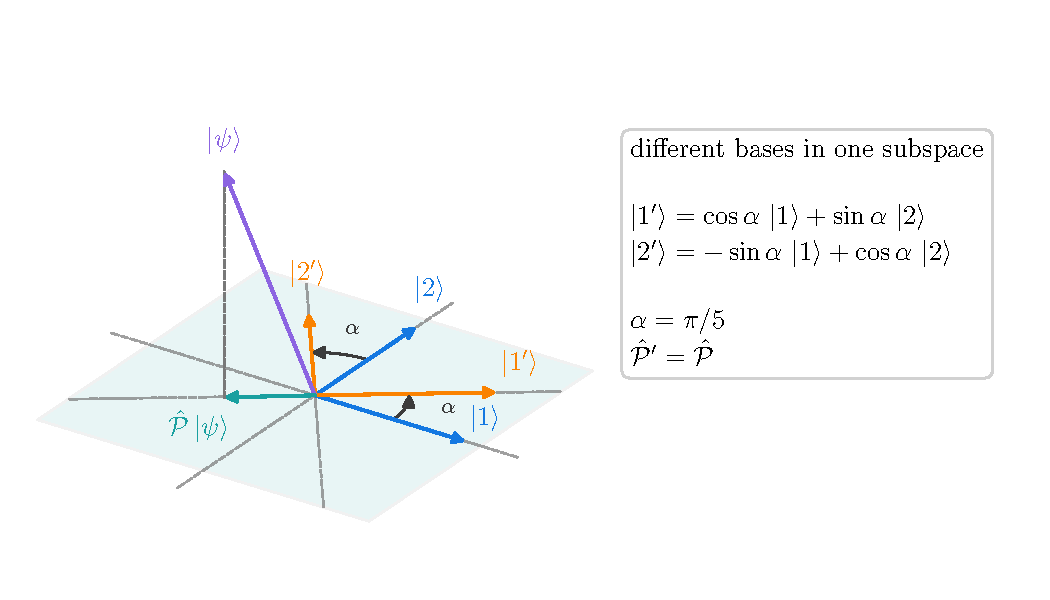
\includegraphics[width=0.8\textwidth]{figures_topo/C.3_subspace_basis.pdf}
    \caption{Two orthonormal bases spanning the same subspace, with the same projector and the same projection of $\ket{\psi}$.}
    \label{fig:subspace_basis_appendix}
\end{figure}

For such a basis, the connection becomes a matrix~\cite{wilczek1984appearance}.
Applying the same derivative as in equation~\eqref{berry_connection_topology} to each pair of basis states gives:

\begin{equation}
\left\{\begin{aligned}
    [\vec{\mathcal{A}}(\vec{k}\,)]_{mn}
    &=\mathrm{i}\bra{u_{m\vec{k}}}\nabla_{\vec{k}}\ket{u_{n\vec{k}}} \\
    \vec{\mathcal{A}}\,'(\vec{k}\,)
    &=U^\dagger(\vec{k}\,)\vec{\mathcal{A}}(\vec{k}\,)U(\vec{k}\,)
    +\mathrm{i}\,U^\dagger(\vec{k}\,)\nabla_{\vec{k}}U(\vec{k}\,)
\end{aligned}\right.
\label{band_subspace_connection_topology}
\end{equation}

here, $m$ and $n$ run over the selected basis states.
The second relation follows by differentiating both the original basis and the matrix $U(\vec{k}\,)$.
For a single state, it reduces to equation~\eqref{berry_connection_gauge_transformation_topology}.
The off-diagonal elements describe the mixing of basis states as $\vec{k}$ changes.
The corresponding curvature is also a matrix:

\begin{equation}
\left\{\begin{aligned}
    \mathcal{F}_{ij}
    &=\partial_{k_i}\mathcal{A}_j-\partial_{k_j}\mathcal{A}_i
    -\mathrm{i}[\mathcal{A}_i,\mathcal{A}_j] \\
    \mathcal{F}'_{ij}&=U^\dagger\mathcal{F}_{ij}U
\end{aligned}\right.
\label{nonabelian_berry_curvature_appendix}
\end{equation}

The commutator accounts for the order of the matrix operations.
This is the non-Abelian generalization of equation~\eqref{abelian_berry_curvature_appendix}~\cite{wilczek1984appearance,xiao2010berry}.
The matrix curvature transforms covariantly under a change of basis; its trace is gauge invariant.
The same differential-form notation applies with matrix-valued coefficients~\cite{hassani2013mathematical}:
$\mathcal{F}=\dif\mathcal{A}-\mathrm{i}\mathcal{A}\wedge\mathcal{A}$.
The ordered matrix products in the wedge term give the commutator in equation~\eqref{nonabelian_berry_curvature_appendix}.
Consequently, assigning independent single-band phases to arbitrary members of a degenerate pair does not characterize the whole subspace.
We must now ask whether these local choices of basis can be joined over the whole Brillouin zone
while respecting time-reversal pairing.
This is a constraint on the full subspace, beyond the phase accumulated around one loop.
Inversion symmetry allows the corresponding $Z_2$ index to be evaluated from parity eigenvalues in chapter~\ref{cha:fundamentals_c}.
We first establish how time reversal acts on the same states.

\newpage
\section{Spinor states and time reversal}
\label{sec:spinors_time_reversal_appendix}

Equation~\eqref{KS_spinor_equation_method} describes the full electronic spinor.
Using the Bloch representation in equation~\eqref{bloch_hamiltonian_topology},
we now express the corresponding cell-periodic state as:

\begin{equation}
    \ket{u_{n\vec{k}}}
    =\ket{u_{n\vec{k},\uparrow}}\otimes\ket{\uparrow}
    +\ket{u_{n\vec{k},\downarrow}}\otimes\ket{\downarrow}
\label{cell_periodic_spinor_topology}
\end{equation}

here, the two spatial components form one spinor state.
They are not two separate occupied bands.
Spin-orbit coupling can mix these components, so spin is not generally a conserved band label.
The time-reversal classification, however, remains applicable when the hamiltonian preserves time-reversal symmetry.

For spin-$1/2$ electrons, we choose the time-reversal operator as:

\begin{equation}
\left\{\begin{aligned}
    \hat{\Theta}&=\mathrm{i}\hat{\sigma}_y\hat{K} \\
    \hat{\Theta}^2&=-\hat{I} \\
    \hat{\Theta}\hat{h}(\vec{k}\,)\hat{\Theta}^{-1}
    &=\hat{h}(-\vec{k}\,)
\end{aligned}\right.
\label{spinful_time_reversal_topology}
\end{equation}

here, $\hat{\sigma}_y$ is the Pauli operator in the chosen spin basis,
$\hat{K}$ takes the complex conjugate in the position and spin representation,
and $\hat{I}$ is the identity operator.
The last relation states the symmetry condition on the hamiltonian.
It applies to the non-magnetic spinful problem considered here;
spin-orbit coupling alone does not break time-reversal symmetry.

Physically, time reversal reverses both the momentum and the spin.
The complex conjugation also means that coefficients in a linear combination are conjugated:

\begin{equation}
    \hat{\Theta}\bigl(c_a\ket{a}+c_b\ket{b}\bigr)
    =c_a^*\hat{\Theta}\ket{a}+c_b^*\hat{\Theta}\ket{b}
\label{time_reversal_antilinearity_topology}
\end{equation}

here, $c_a$ and $c_b$ are complex coefficients.
This property is called antilinearity.
In the chosen spin basis, the convention in equation~\eqref{spinful_time_reversal_topology} gives
$\hat{\Theta}\ket{\uparrow}=-\ket{\downarrow}$ and
$\hat{\Theta}\ket{\downarrow}=\ket{\uparrow}$.
Applying time reversal twice therefore returns either spin state with a minus sign,
which explains $\hat{\Theta}^2=-\hat{I}$.
The two components of one spinor should consequently be distinguished from its time-reversed partner, which is another complete state.

The operator $\hat{\Theta}$ preserves norms while conjugating inner products, and is therefore antiunitary.
For any two states, it satisfies
$\braket{\hat{\Theta}a|\hat{\Theta}b}=\braket{b|a}$.
To apply this relation at a time-reversal invariant momentum (TRIM), we use a full Bloch state $\ket{\psi}$.
At such a point, the reversed wave vector differs from the original by a reciprocal-lattice vector,
so both states have the same phases under lattice translations.
Taking $\ket{a}=\ket{\psi}$ and $\ket{b}=\hat{\Theta}\ket{\psi}$ gives:

\begin{equation}
    \braket{\hat{\Theta}\psi|\psi}
    =\braket{\hat{\Theta}\psi|\hat{\Theta}^2\psi}
    =-\braket{\hat{\Theta}\psi|\psi}
\label{kramers_orthogonality_topology}
\end{equation}

Consequently, $\braket{\hat{\Theta}\psi|\psi}=0$.
Time-reversal symmetry also gives $\hat{h}\hat{\Theta}=\hat{\Theta}\hat{h}$ for the full hamiltonian.
If $\hat{h}\ket{\psi}=E\ket{\psi}$, its partner therefore satisfies:

\begin{equation}
    \hat{h}\hat{\Theta}\ket{\psi}
    =\hat{\Theta}\hat{h}\ket{\psi}
    =E\hat{\Theta}\ket{\psi}
\label{kramers_equal_energy_topology}
\end{equation}

here, the energy $E$ is real because $\hat{h}$ is Hermitian.
At a wave vector equivalent to its negative, $\ket{\psi}$ and $\hat{\Theta}\ket{\psi}$
therefore represent orthogonal states with the same energy and wave vector.
These states form a Kramers pair.
Removing the same Bloch factor from both states preserves their orthogonality,
so the pairing also supplies two orthogonal cell-periodic states at this representative wave vector.
At a general wave vector, time reversal instead relates a state at $\vec{k}$ to an equal-energy state at $-\vec{k}$.
